\chapter{Лабораторная работа 1 \\
Статические характеристики и цепи смещения транзисторных усилителей}

Цель работы: научиться измерять и анализировать статические характеристики усилителей на биполярном и полевом транзисторах, научиться проектировать схемы смещения усилителей на биполярном и полевом транзисторах, получить навыки работы со средой моделирования Advanced Design System.

\section{Техническое задание}

Определить выходные статические характеристики биполярного (HBFP0420) и полевого (MGF2148) транзисторов. Выбрать рабочую точку и расчитать цепь смещения.

\section{Выполнение работы}

\subsection{Измерение выходных статических характеристик биполярного транзистора}

Для измерения выходных статических характеристик биполярного транзистора необходимо собрать модель, показанную на рис.~\ref{fig:bias_circuits_bipolar_schematic_1}.

\begin{figure}[!ht]
    \centering
    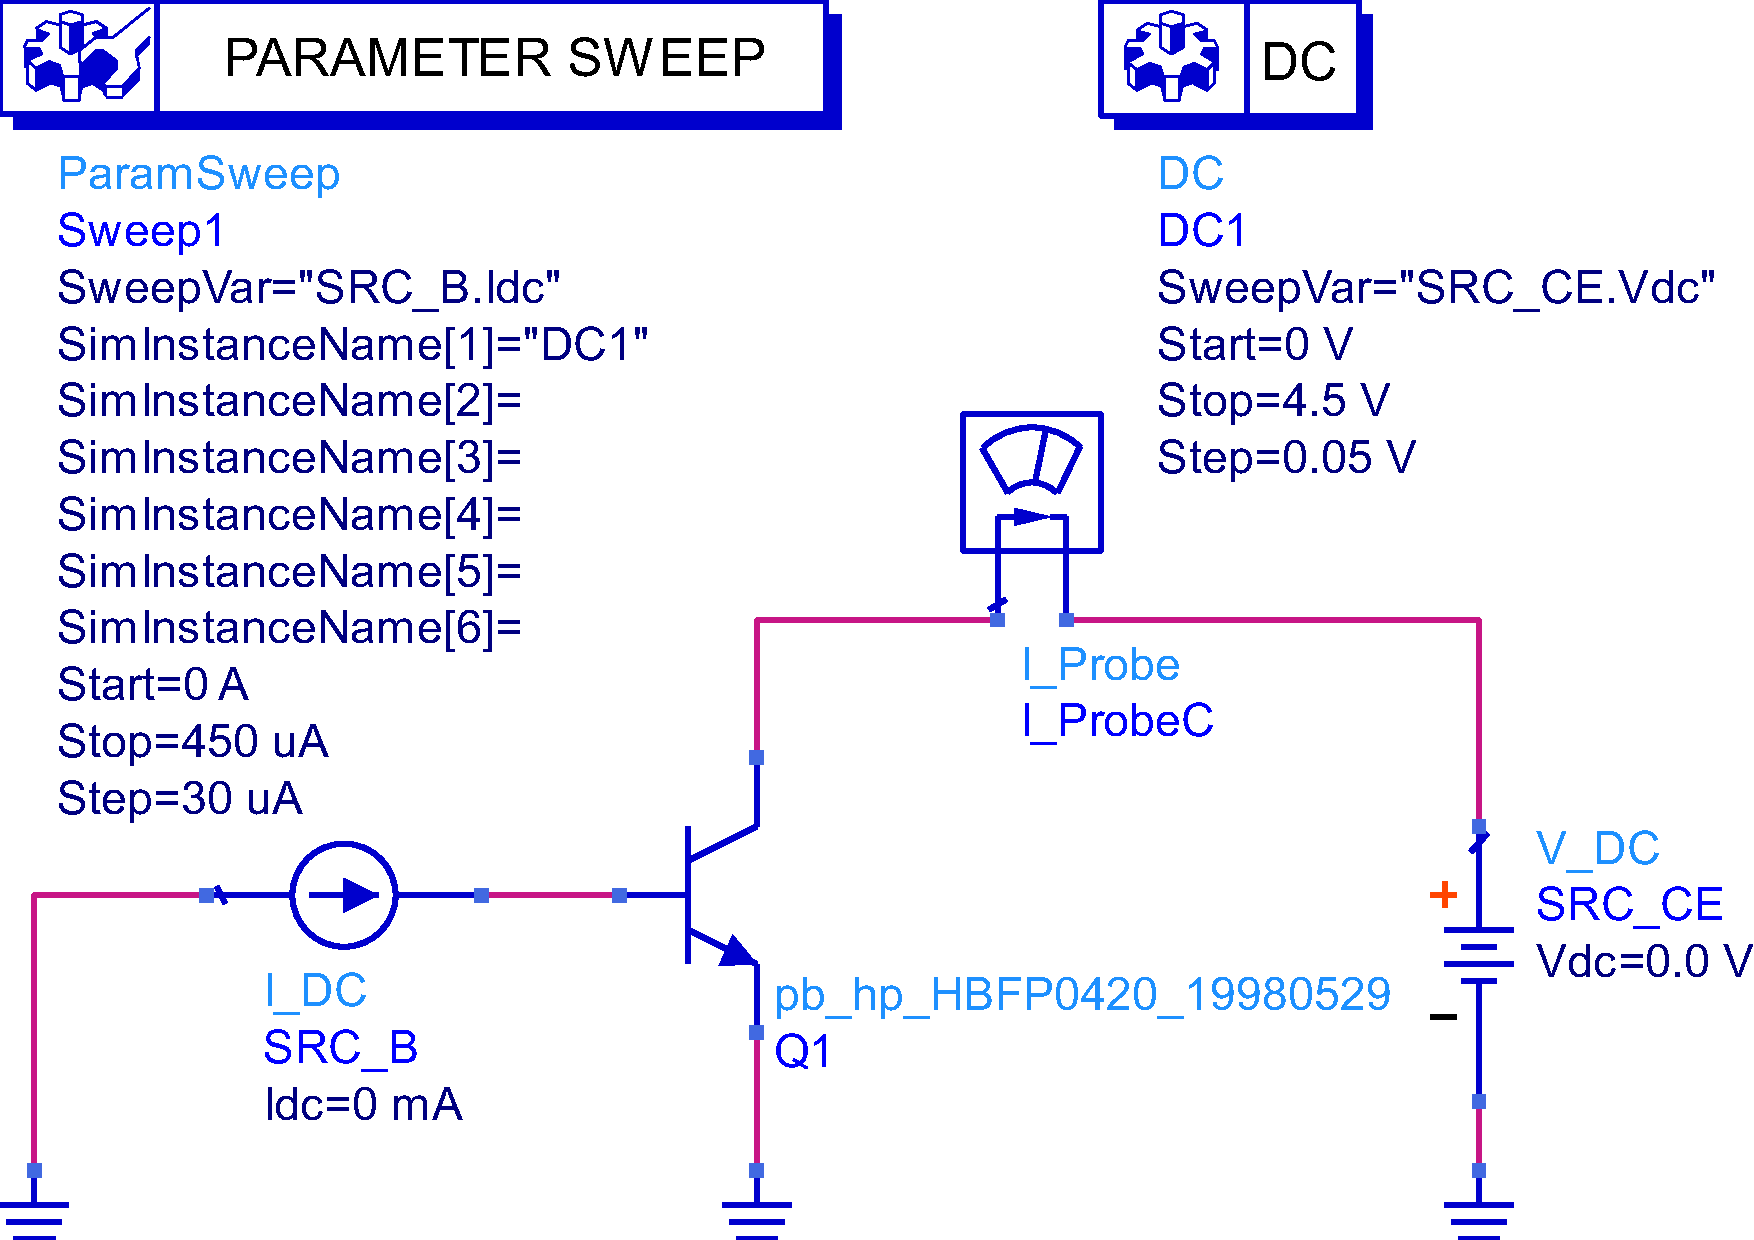
\includegraphics[width=0.7\textwidth]{bias_circuits_bipolar_schematic_1}
    \caption{Схема для измерения выходных статических характеристик биполярного транзистора}%
    \label{fig:bias_circuits_bipolar_schematic_1}
\end{figure}

Источник постоянного напряжения \elementname{SRC\_CE} задает напряжение коллектор-эмиттер и источник постоянного тока \elementname{SRC\_B} задает ток базы.
Ток коллектора измеряется с помощью \elementname{I\_ProbeC}.
В свойствах симулятора DC1 задается диапазон изменения напряжения коллектор-эмиттер (независимая переменная) и в дополнительном блоке \elementname{Ib\_Sweep} задается набор тока базы.
Предел напряжения коллектор-эмиттер брать от 0 В до предельно допустимого из рекомендаций производителя. Предел тока базы брать от 0 А до предельно допустимого из рекомендаций производителя.
Измеряемое семейство графиков будет выглядеть как показано на рис.~\ref{fig:bias_circuits_bipolar_data_display_1}.

\begin{figure}[!ht]
    \centering
    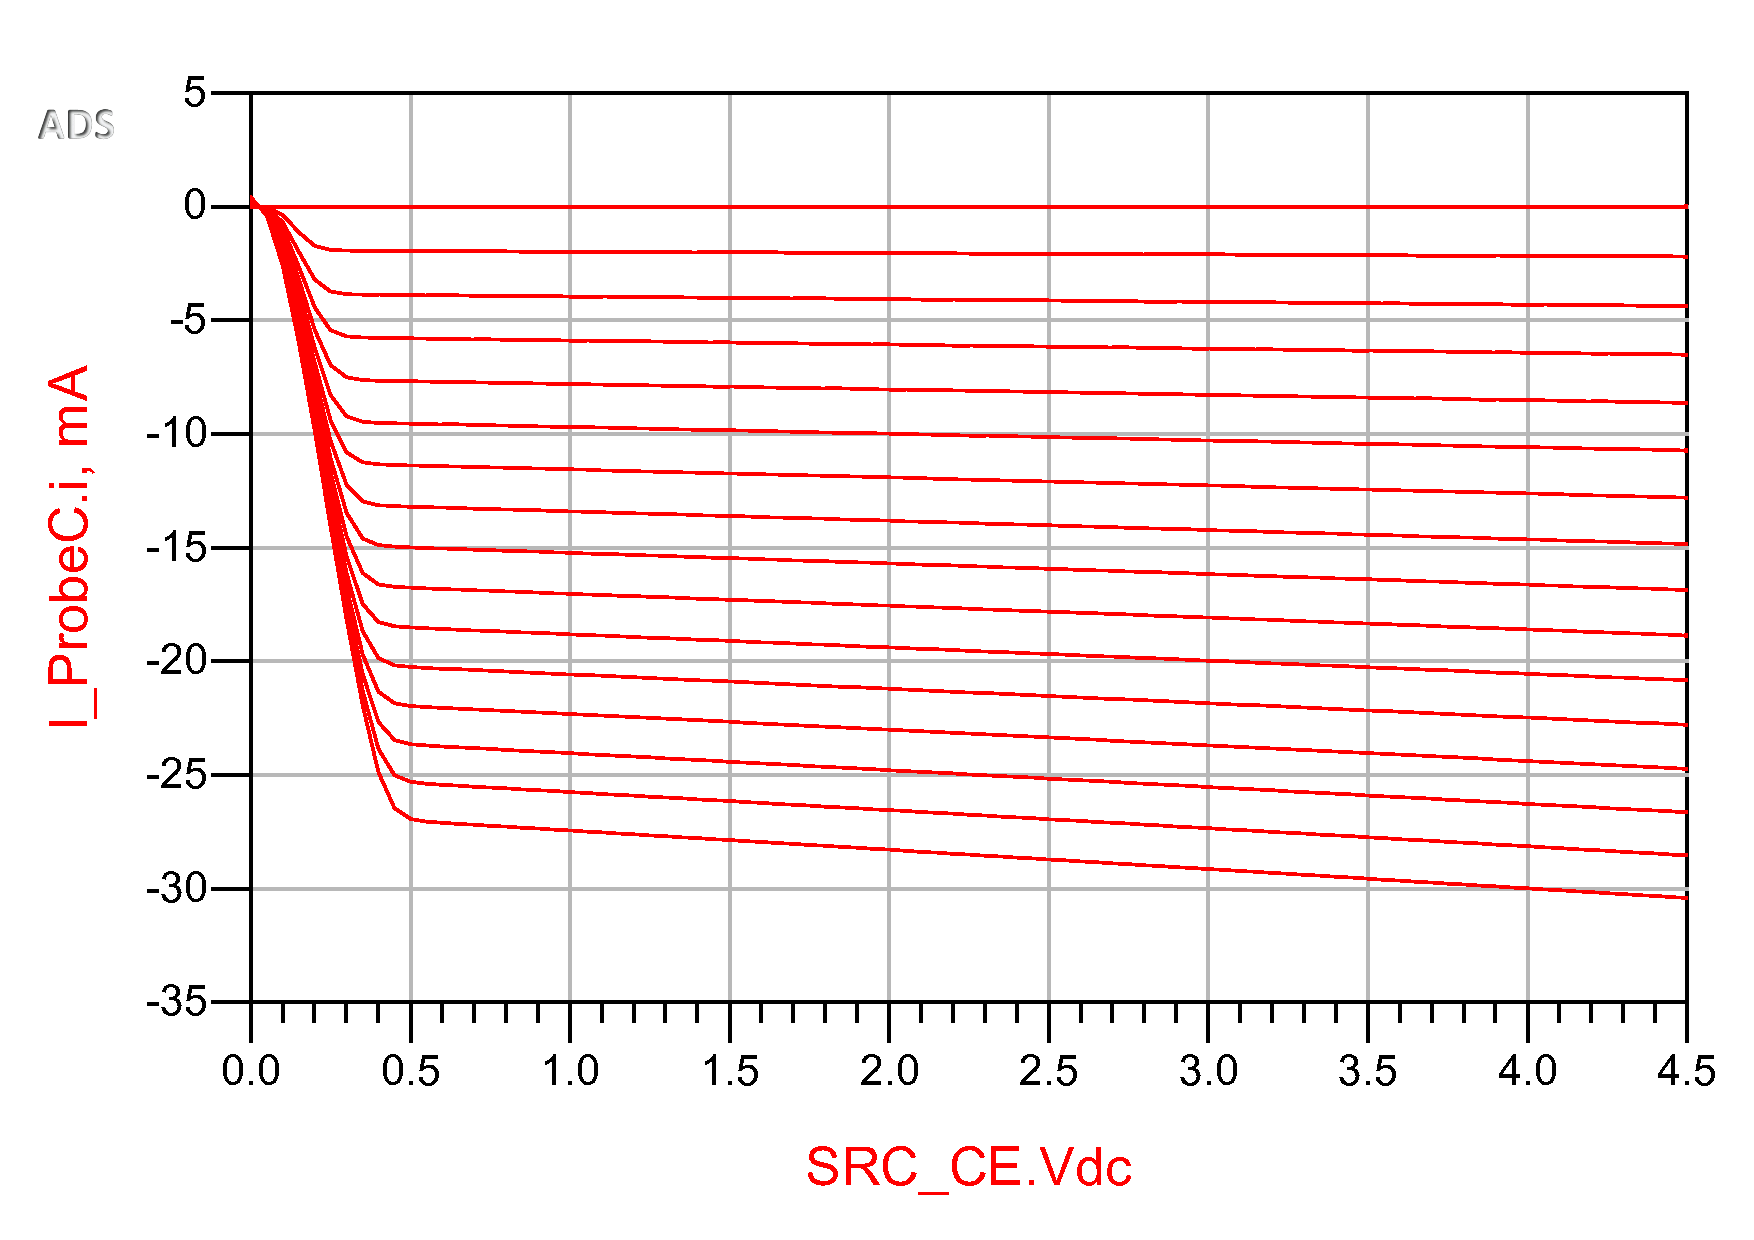
\includegraphics[width=0.8\textwidth]{bias_circuits_bipolar_data_display_1}
    \caption{Выходные статические характеристики биполярного транзистора}%
    \label{fig:bias_circuits_bipolar_data_display_1}
\end{figure}

\subsection{Измерение выходных статических характеристик полевого транзистора}

Для измерения выходных статических характеристик биполярного транзистора необходимо собрать модель, показанную на рис.~\ref{fig:bias_circuits_field_schematic}.

\begin{figure}[!ht]
    \centering
    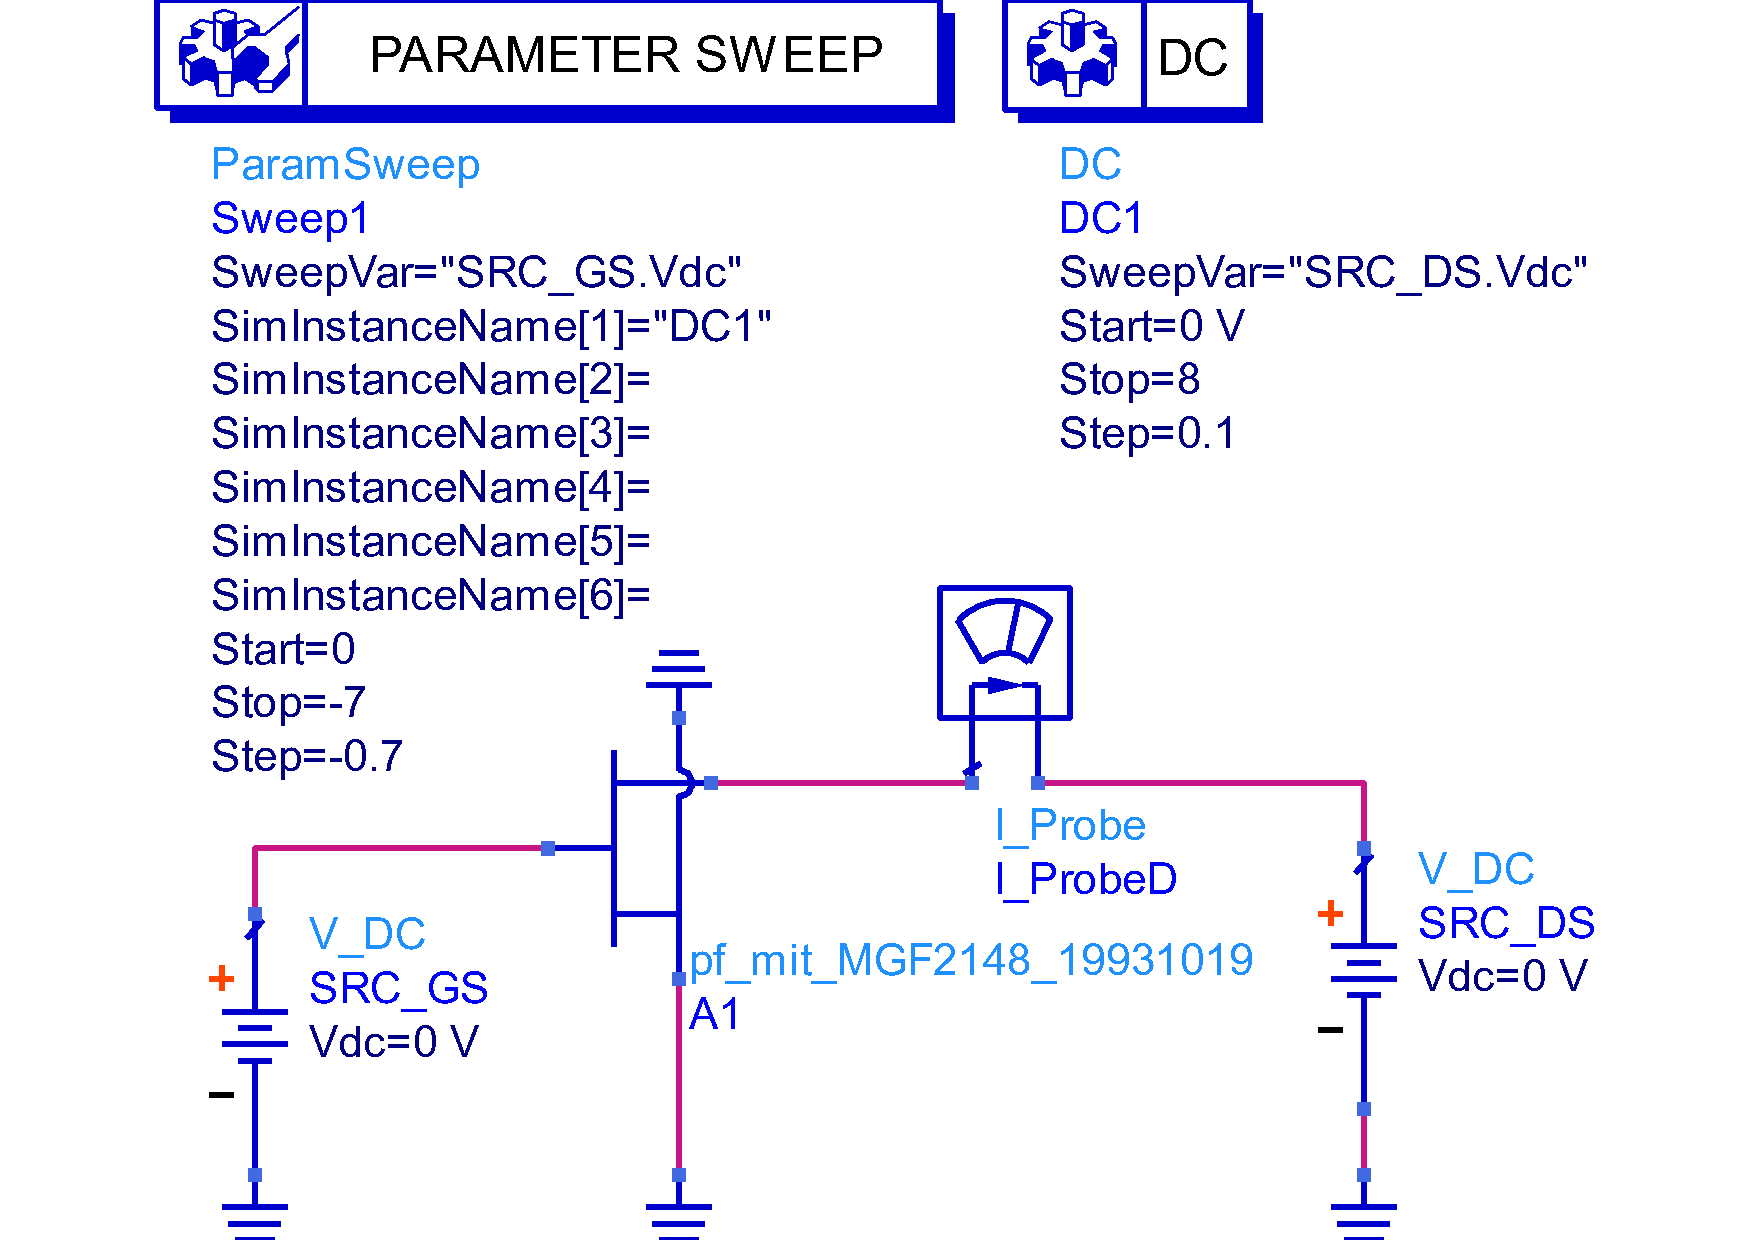
\includegraphics[width=0.8\textwidth]{bias_circuits_field_schematic}
    \caption{Схема для измерения выходных статических характеристик полевого транзистора}%
    \label{fig:bias_circuits_field_schematic}
\end{figure}

Два источника постоянного напряжения \elementname{SRC\_GS} и \elementname{SRC\_DS} задают напряжения затвор-исток (gate-source) и сток-исток (drain-source) соответственно.
Ток стока измеряется с помощью \elementname{I\_ProbeD}. В свойствах симулятора \elementname{DC1} задается диапазон изменения напряжения сток-исток (независимая переменная) и в дополнительном блоке \elementname{VGS\_Sweep} задается набор напряжений затвор-исток.

Предел напряжения сток-исток брать от 0~В до предельно допустимого из рекомендаций производителя. Предел напряжения затвор-исток тока базы брать от предельно допустимого из рекомендаций производителя до 0~В.

Измеряемое семейство графиков будет выглядеть как показано на рис.~\ref{fig:bias_circuits_field_data_display}.

\begin{figure}[!ht]
    \centering
    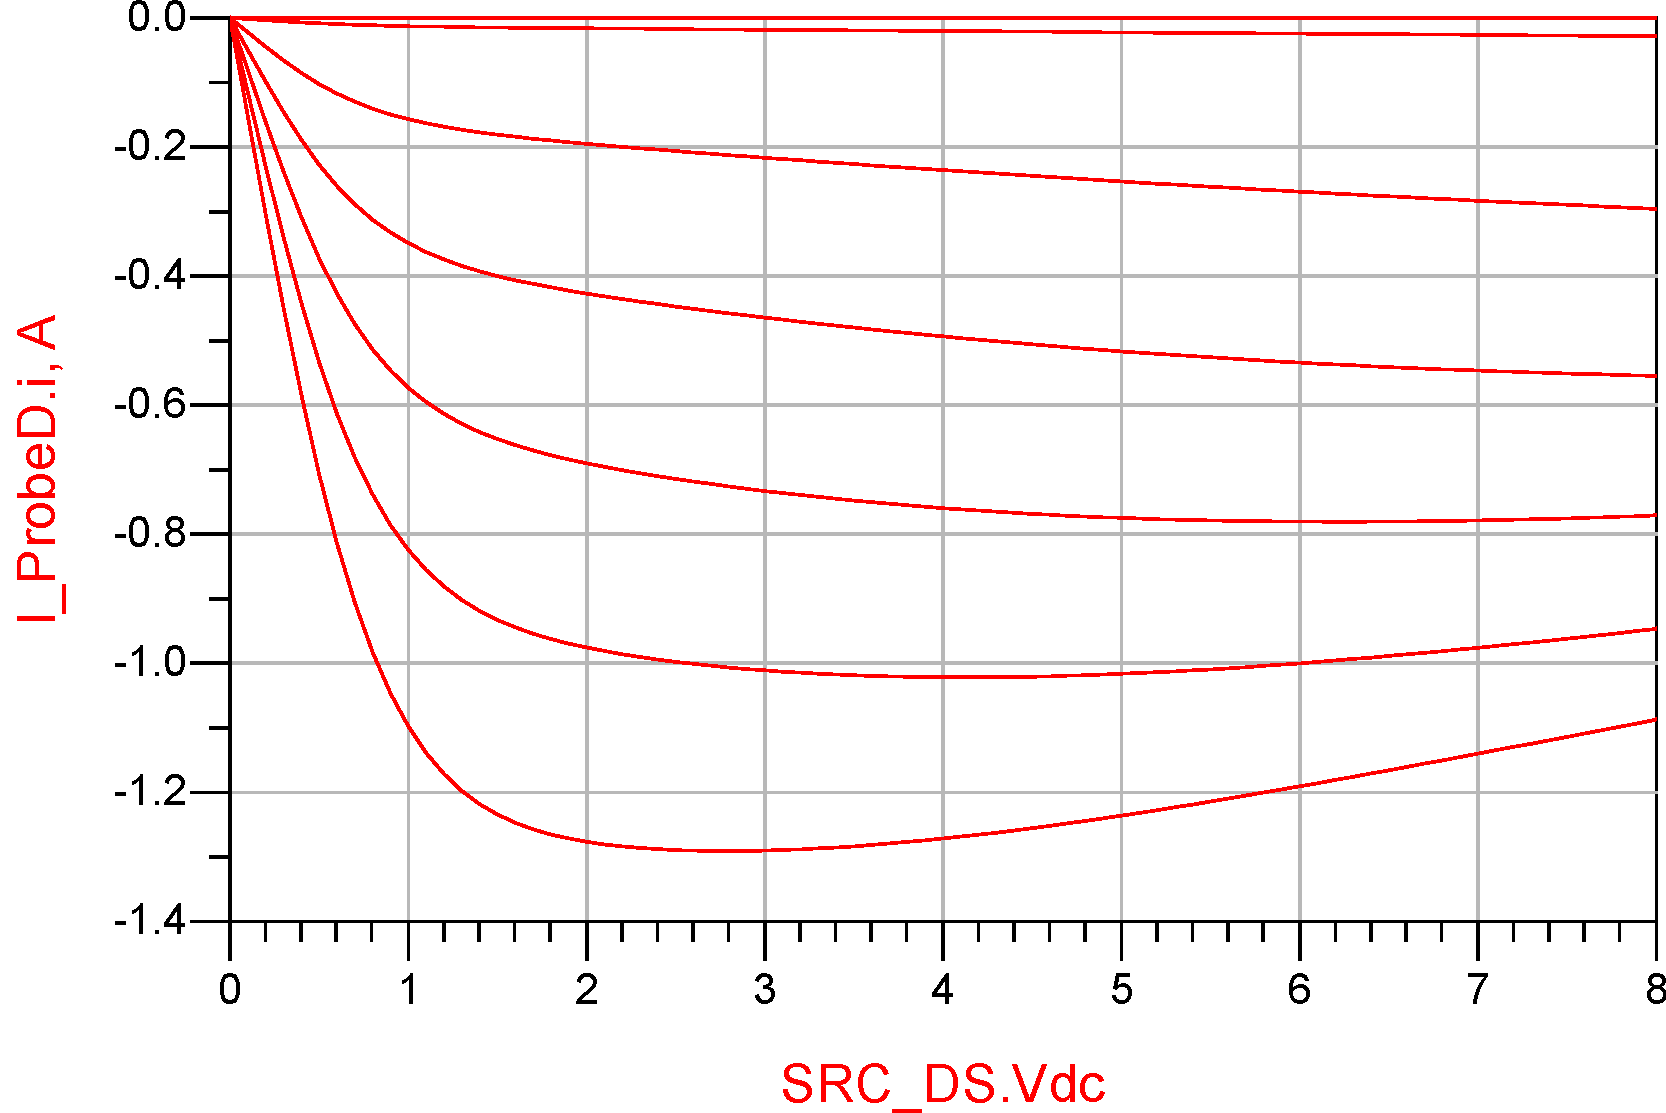
\includegraphics[width=0.8\textwidth]{bias_circuits_field_data_display}
    \caption{Выходные статические характеристики полевого транзистора}%
    \label{fig:bias_circuits_field_data_display}
\end{figure}
\subsection{Расчёт цепей смещения биполярного транзистора}

Для расчёта цепи смещения по постоянному току собрать схему на рис.~\ref{fig:bias_circuits_bipolar_bias_schematic_1}.
\begin{figure}[!ht]
    \centering
    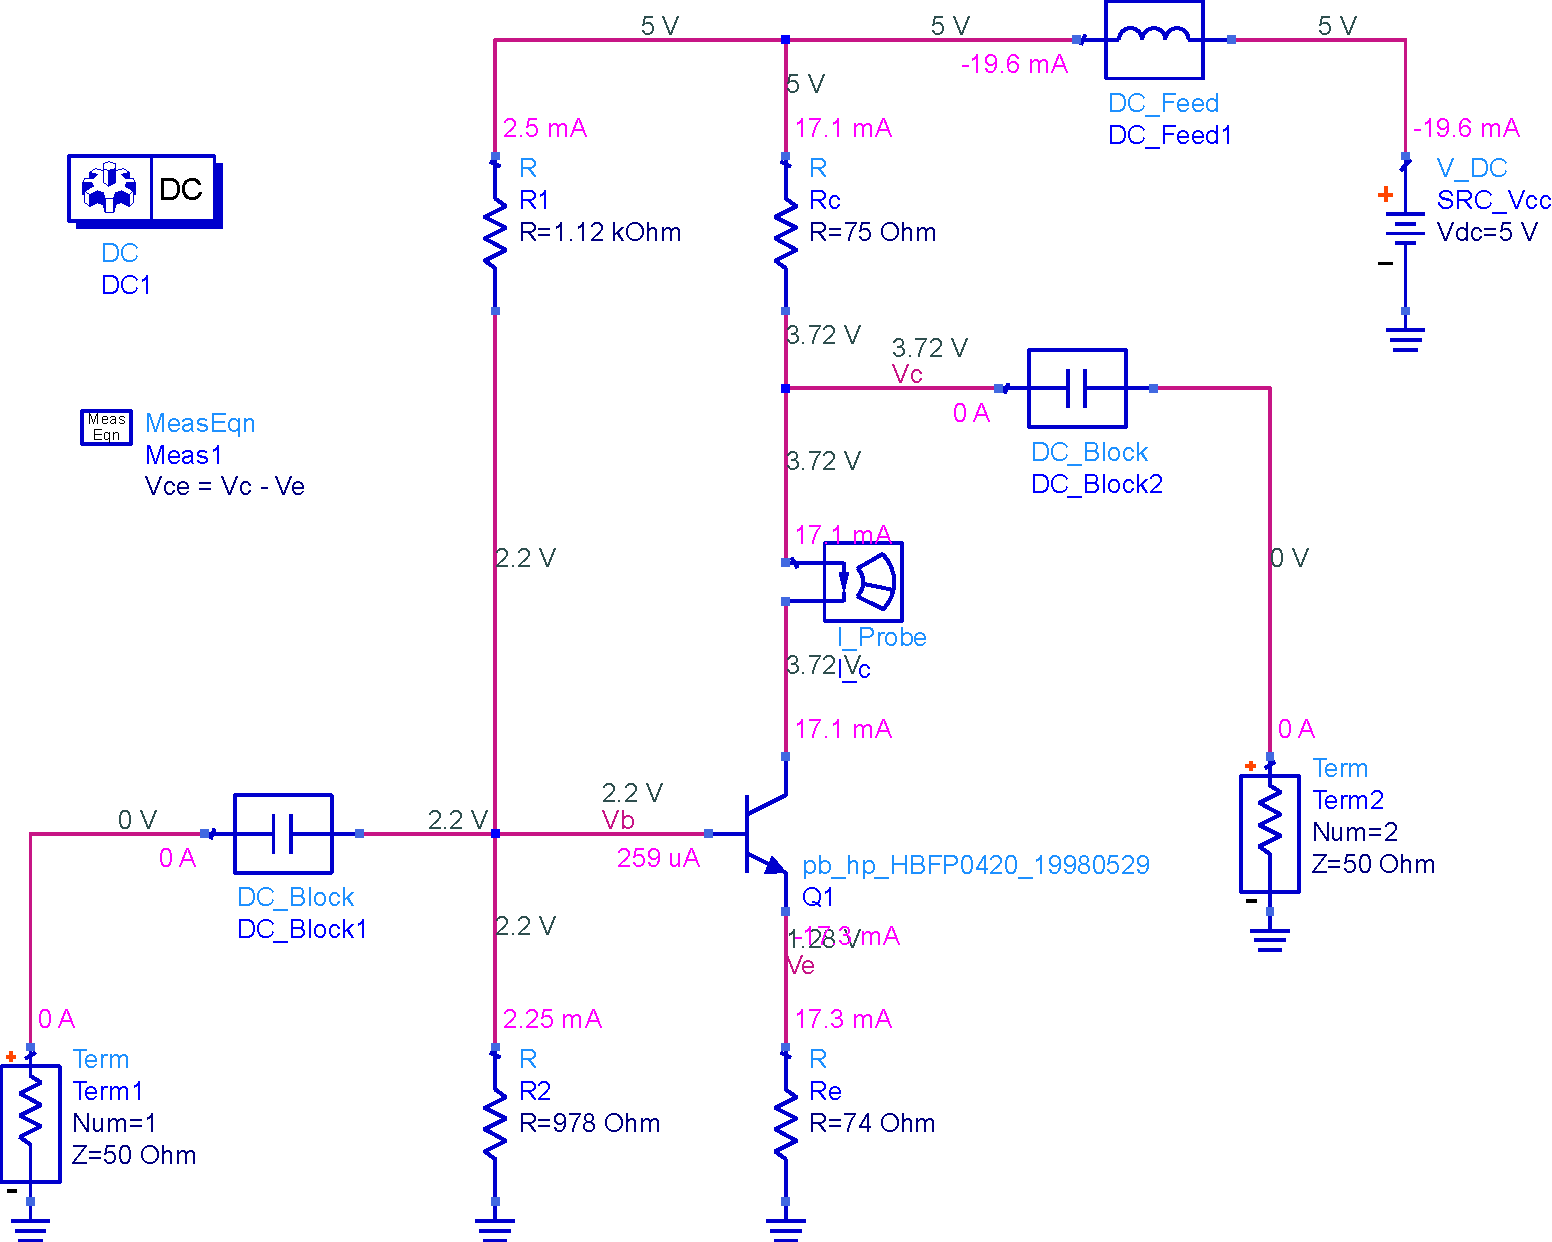
\includegraphics[width=0.8\textwidth]{bias_circuits_bipolar_bias_schematic_1.pdf}
    \caption{Цепь смещения по постоянному току}%
    \label{fig:bias_circuits_bipolar_bias_schematic_1}
\end{figure}

Транзистор можно взять из библиотеки \elementname{RF Transistor Library} или забить параметры в модель \elementname{BJT\_Model}.
Свойства транзисторов можно посмотреть в рекомендации производителя на компонент.
В расчете участвуют точка смещения ($U_\text{КЭ}$ и $I_\text{К}$) и коэффициент усиления по току $\beta$ или $h_{fe}$.
Рабочую точку выбрать одну из рекомендованных производителем.
Рекомендованные рабочие точки указаны в рекомендации производителя как точки \emph{optimum noise figure} и \emph{optimum P1db} (либо \emph{optimum GA}).
Напряжение источника $V_{CC}$ брать из ряда 5, 7, 10, 12, 15, 20, 25~В, но не менее, чем 2--3 напряжения коллектор-эмиттер $U_\text{КЭ}$ в рабочей точке.

Расчёт идёт в следующем порядке (предполагается одинаковое падение напряжения $V_{CC} - V_{CE}$ на $R_C$ и $R_E$):
\begin{enumerate}
    \item потенциал в колекторе $V_C = V_{CC} - \frac{V_{CC} - V_{CE}}{2}$;
    \item потенциал в эмиттере $V_E = \frac{V_{CC} - V_{CE}}{2}$;
    \item сопротивление $R_C = \frac{V_{CC} - V_C}{I_C}$, сопротивление $R_E = \frac{V_E}{I_E}$;
    \item потенциал в базе $V_B = V_{BE} + V_E$, где $V_E \approx 0.7 \text{~В}$ для биполярных транзисторов;
    \item ток базы $I_B = \frac{I_C}{\beta}$;
    \item исходя из эмпирического правила $I_{R_1} = 10 I_B$ и $I_{R_2} = 9 I_B$ сопротивления $R_1 = \frac{V_{CC} - V_B}{10 I_B}$ и $R_2 = \frac{V_B}{9 I_B}$.
\end{enumerate}

Проведём расчёт непосредственно в ADS (Рис.~\ref{fig:bias_circuits_bipolar_bias_data_display_1}).
\begin{figure}[!ht]
    \centering
    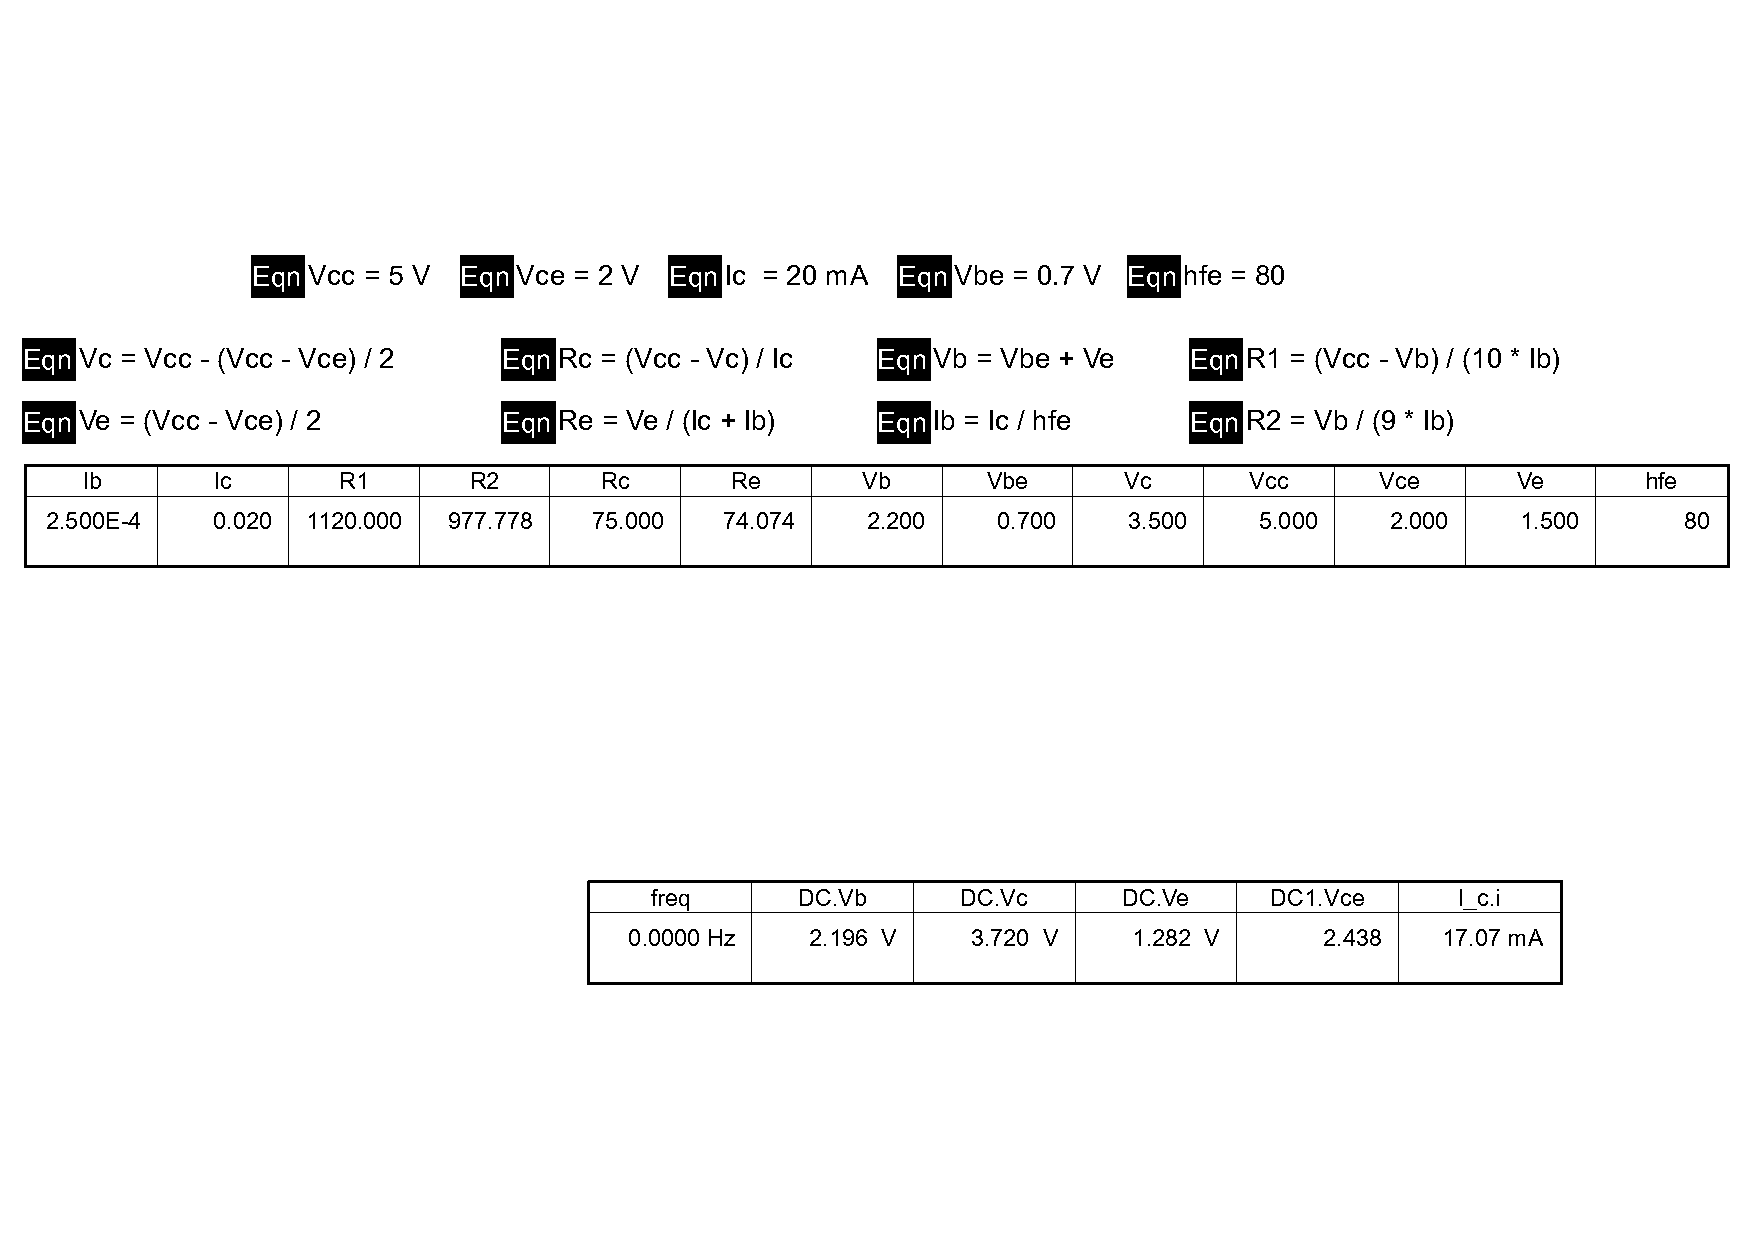
\includegraphics[width=0.9\textwidth]{bias_circuits_bipolar_bias_data_display_1.pdf}
    \caption{Расчёт цепи смещения биполярного транзистора}%
    \label{fig:bias_circuits_bipolar_bias_data_display_1}
\end{figure}

\subsection{Расчёт цепей смещения полевого транзистора}

Для расчёта цепи смещения по постоянному току собрать схему на рис.~\ref{fig:bias_circuits_field_bias_schematic_1}.
\begin{figure}[!ht]
    \centering
    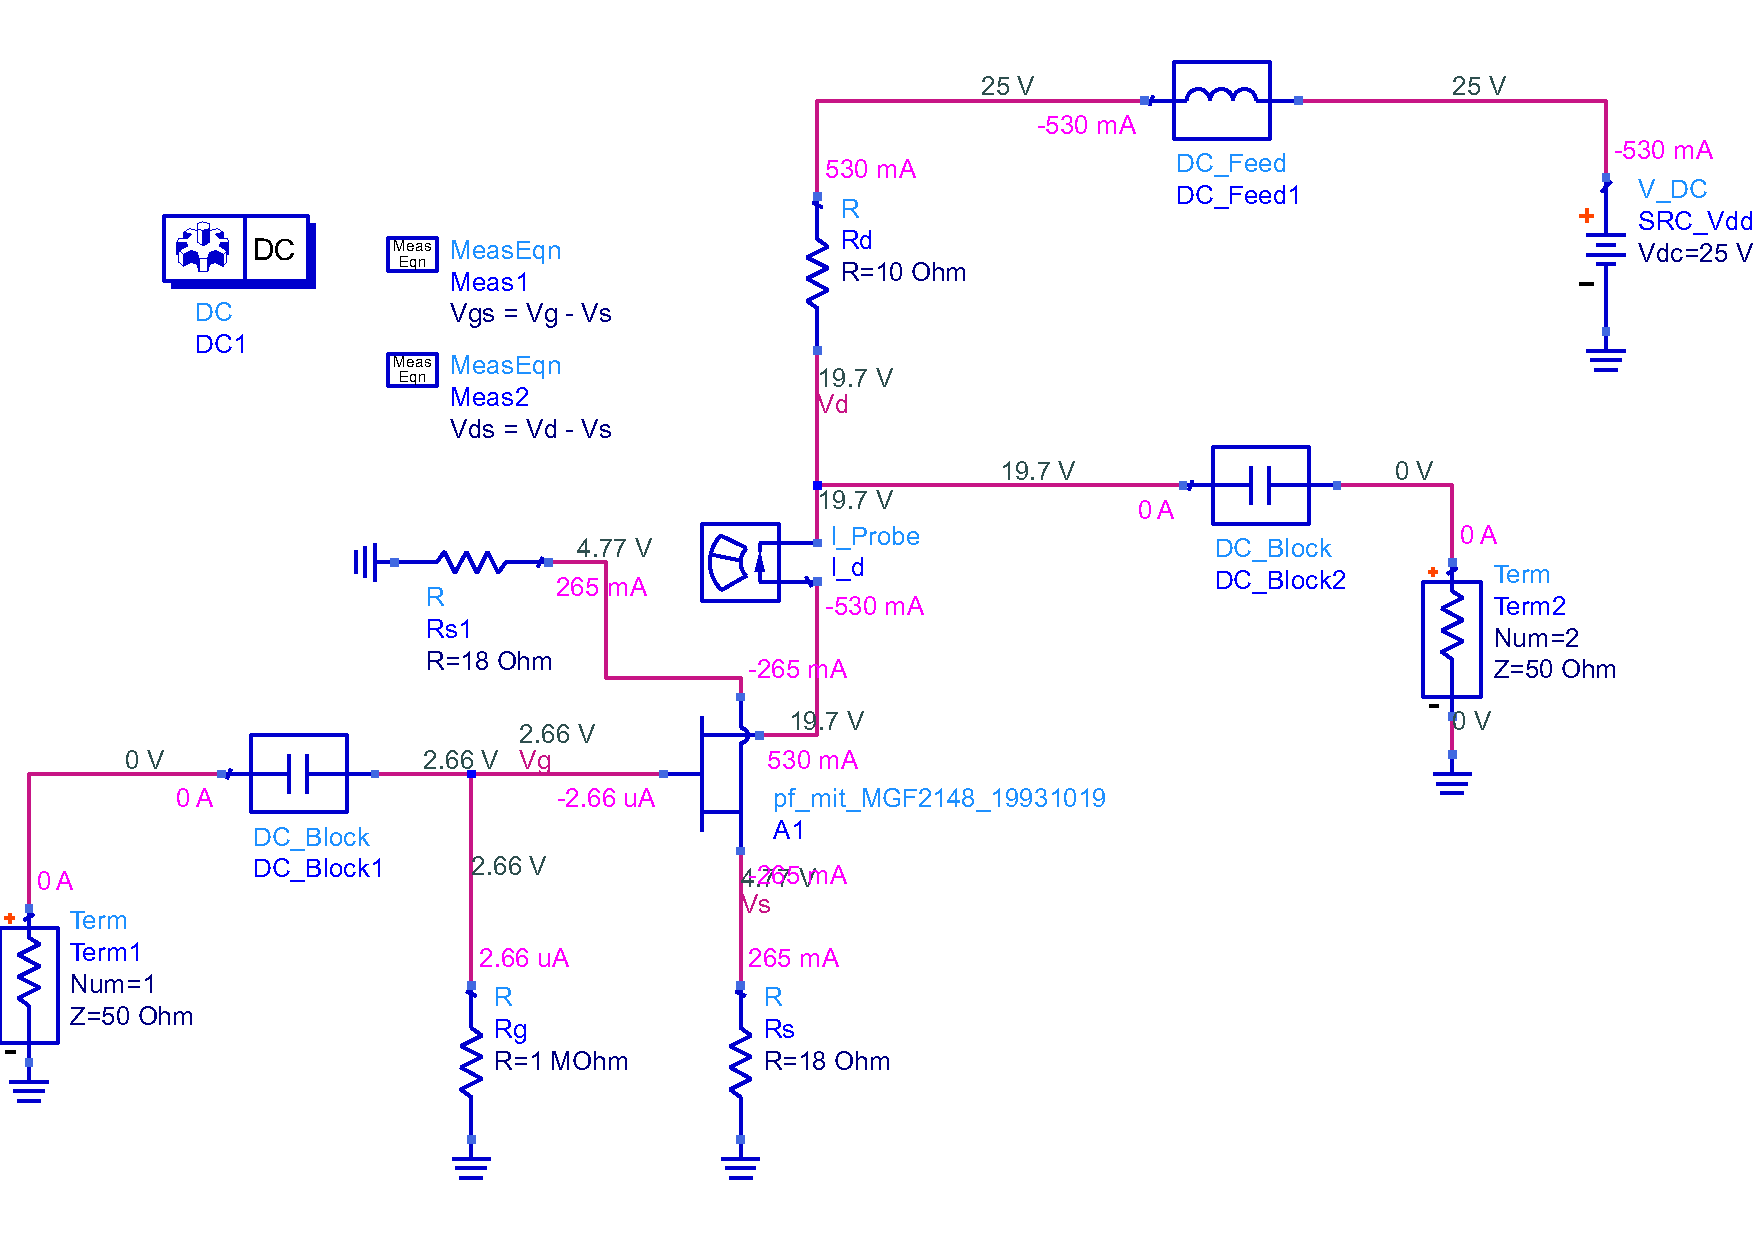
\includegraphics[width=0.8\textwidth]{bias_circuits_field_bias_schematic_1.pdf}
    \caption{Цепь смещения по постоянному току}%
    \label{fig:bias_circuits_field_bias_schematic_1}
\end{figure}

Транзистор можно взять из библиотеки \elementname{RF Transistor Library} или забить параметры в модель \elementname{JFET\_Model}.
Свойства транзисторов можно посмотреть в рекомендации производителя на компонент.
В расчете участвуют точка смещения ($U_\text{СИ}$ и $I_\text{С}$), свойства транзистора --- ток насыщения $I_{DSS}$ и напряжение отсечки $U_{GS(off)}$.
Рабочую точку выбрать одну из рекомендованных производителем.
Рекомендованные рабочие точки указаны в рекомендации производителя как точки \emph{optimum noise figure} и \emph{optimum P1db} (либо \emph{optimum GA}).
Напряжение источника $V_{CC}$ брать из ряда 3.3, 5, 7, 10, 12, 15, 20, 25~В, но не менее, чем 1.5--2.5 напряжения сток-исток $U_\text{СИ}$ в рабочей точке.

Расчёт идёт в следующем порядке (предполагается одинаковое падение напряжения $V_{CC} - V_{CE}$ на $R_C$ и $R_E$):
\begin{enumerate}
    \item через резистор $R_G$ ток не идёт, поэтому его следует выбрать порядка 1~МОм;
    \item используя формулу $I_{DS} = I_{DSS} {\left(1 - \frac{V_{GS}}{V_{GS(off)}}\right)}^2$ определяют напряжение затвор-исток $V_{GS}$ (либо по графику выходных статических характеристик), принимая во внимание, что $V_{GS} < 0$;
    \item т.к. в эквивалентной модели по постоянному току потенциал затвора равен $V_G = 0$, то можно определить потенциал в истоке $V_S = V_G - V_{GS} = -V_{GS}$;
    \item ток истока совпадает с током стока $I_S = I_D$, следовательно, сопротивление истока определяется как $R_S = \frac{V_S}{I_S} = \frac{V_S}{I_D}$;
    \item падение напряжения на резисторе $R_D$ определяется как $V_{DD} - V_{DS} - V_{S}$, соответственно его номинал $R_D = \frac{(V_{DD} - V_{DS} - V_S)}{I_D}$.
\end{enumerate}

Проведём расчёт непосредственно в ADS (Рис.~\ref{fig:bias_circuits_field_bias_data_display_1}).
\begin{figure}[!ht]
    \centering
    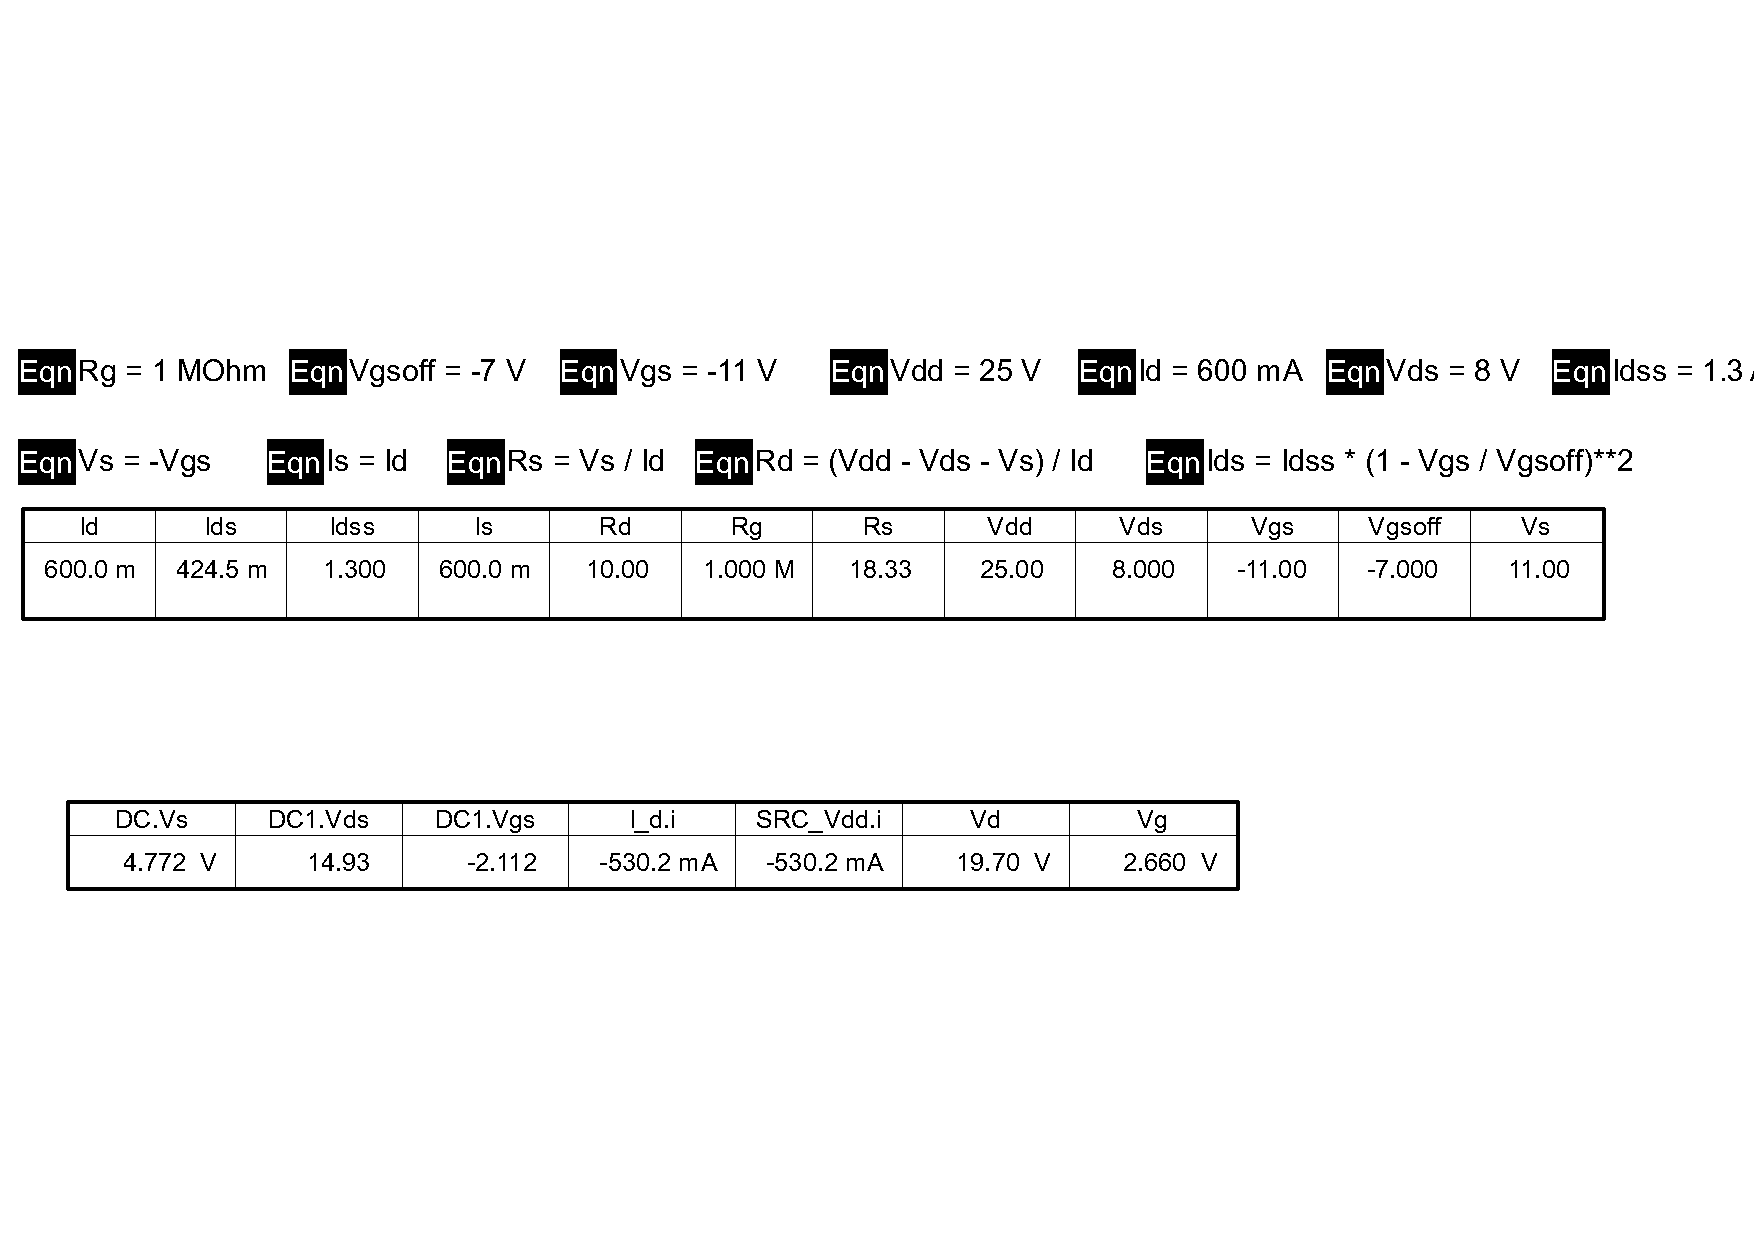
\includegraphics[width=0.9\textwidth]{bias_circuits_field_bias_data_display_1.pdf}
    \caption{Расчёт цепи смещения полевого транзистора}%
    \label{fig:bias_circuits_field_bias_data_display_1}
\end{figure}
